\chapter{Architectural design}

\section{Overview}


\section{High level components and their interactions}


\section{Lower level modules view}


\section{Deployment view}
Two artifacts are going to be deployed, each with a different target.

The first will be the \emph{server} artifact, which will operate on a cluster of servers and will be composed of all components from the, as mentioned, Business and Web tiers. These will form the server side of the whole system, and will interface with their respectived database components from the Data tier.

The second will be the \emph{client} artifact, in the form of the \mts{} mobile app, which will run on smartphones and interface with the \emph{server} artifact with the discussed methodologies, and will be made up of all previously highlighted components belonging to the Client tier.

\section{Runtime view}


\section{Component interfaces}
\begin{figure}
\centering
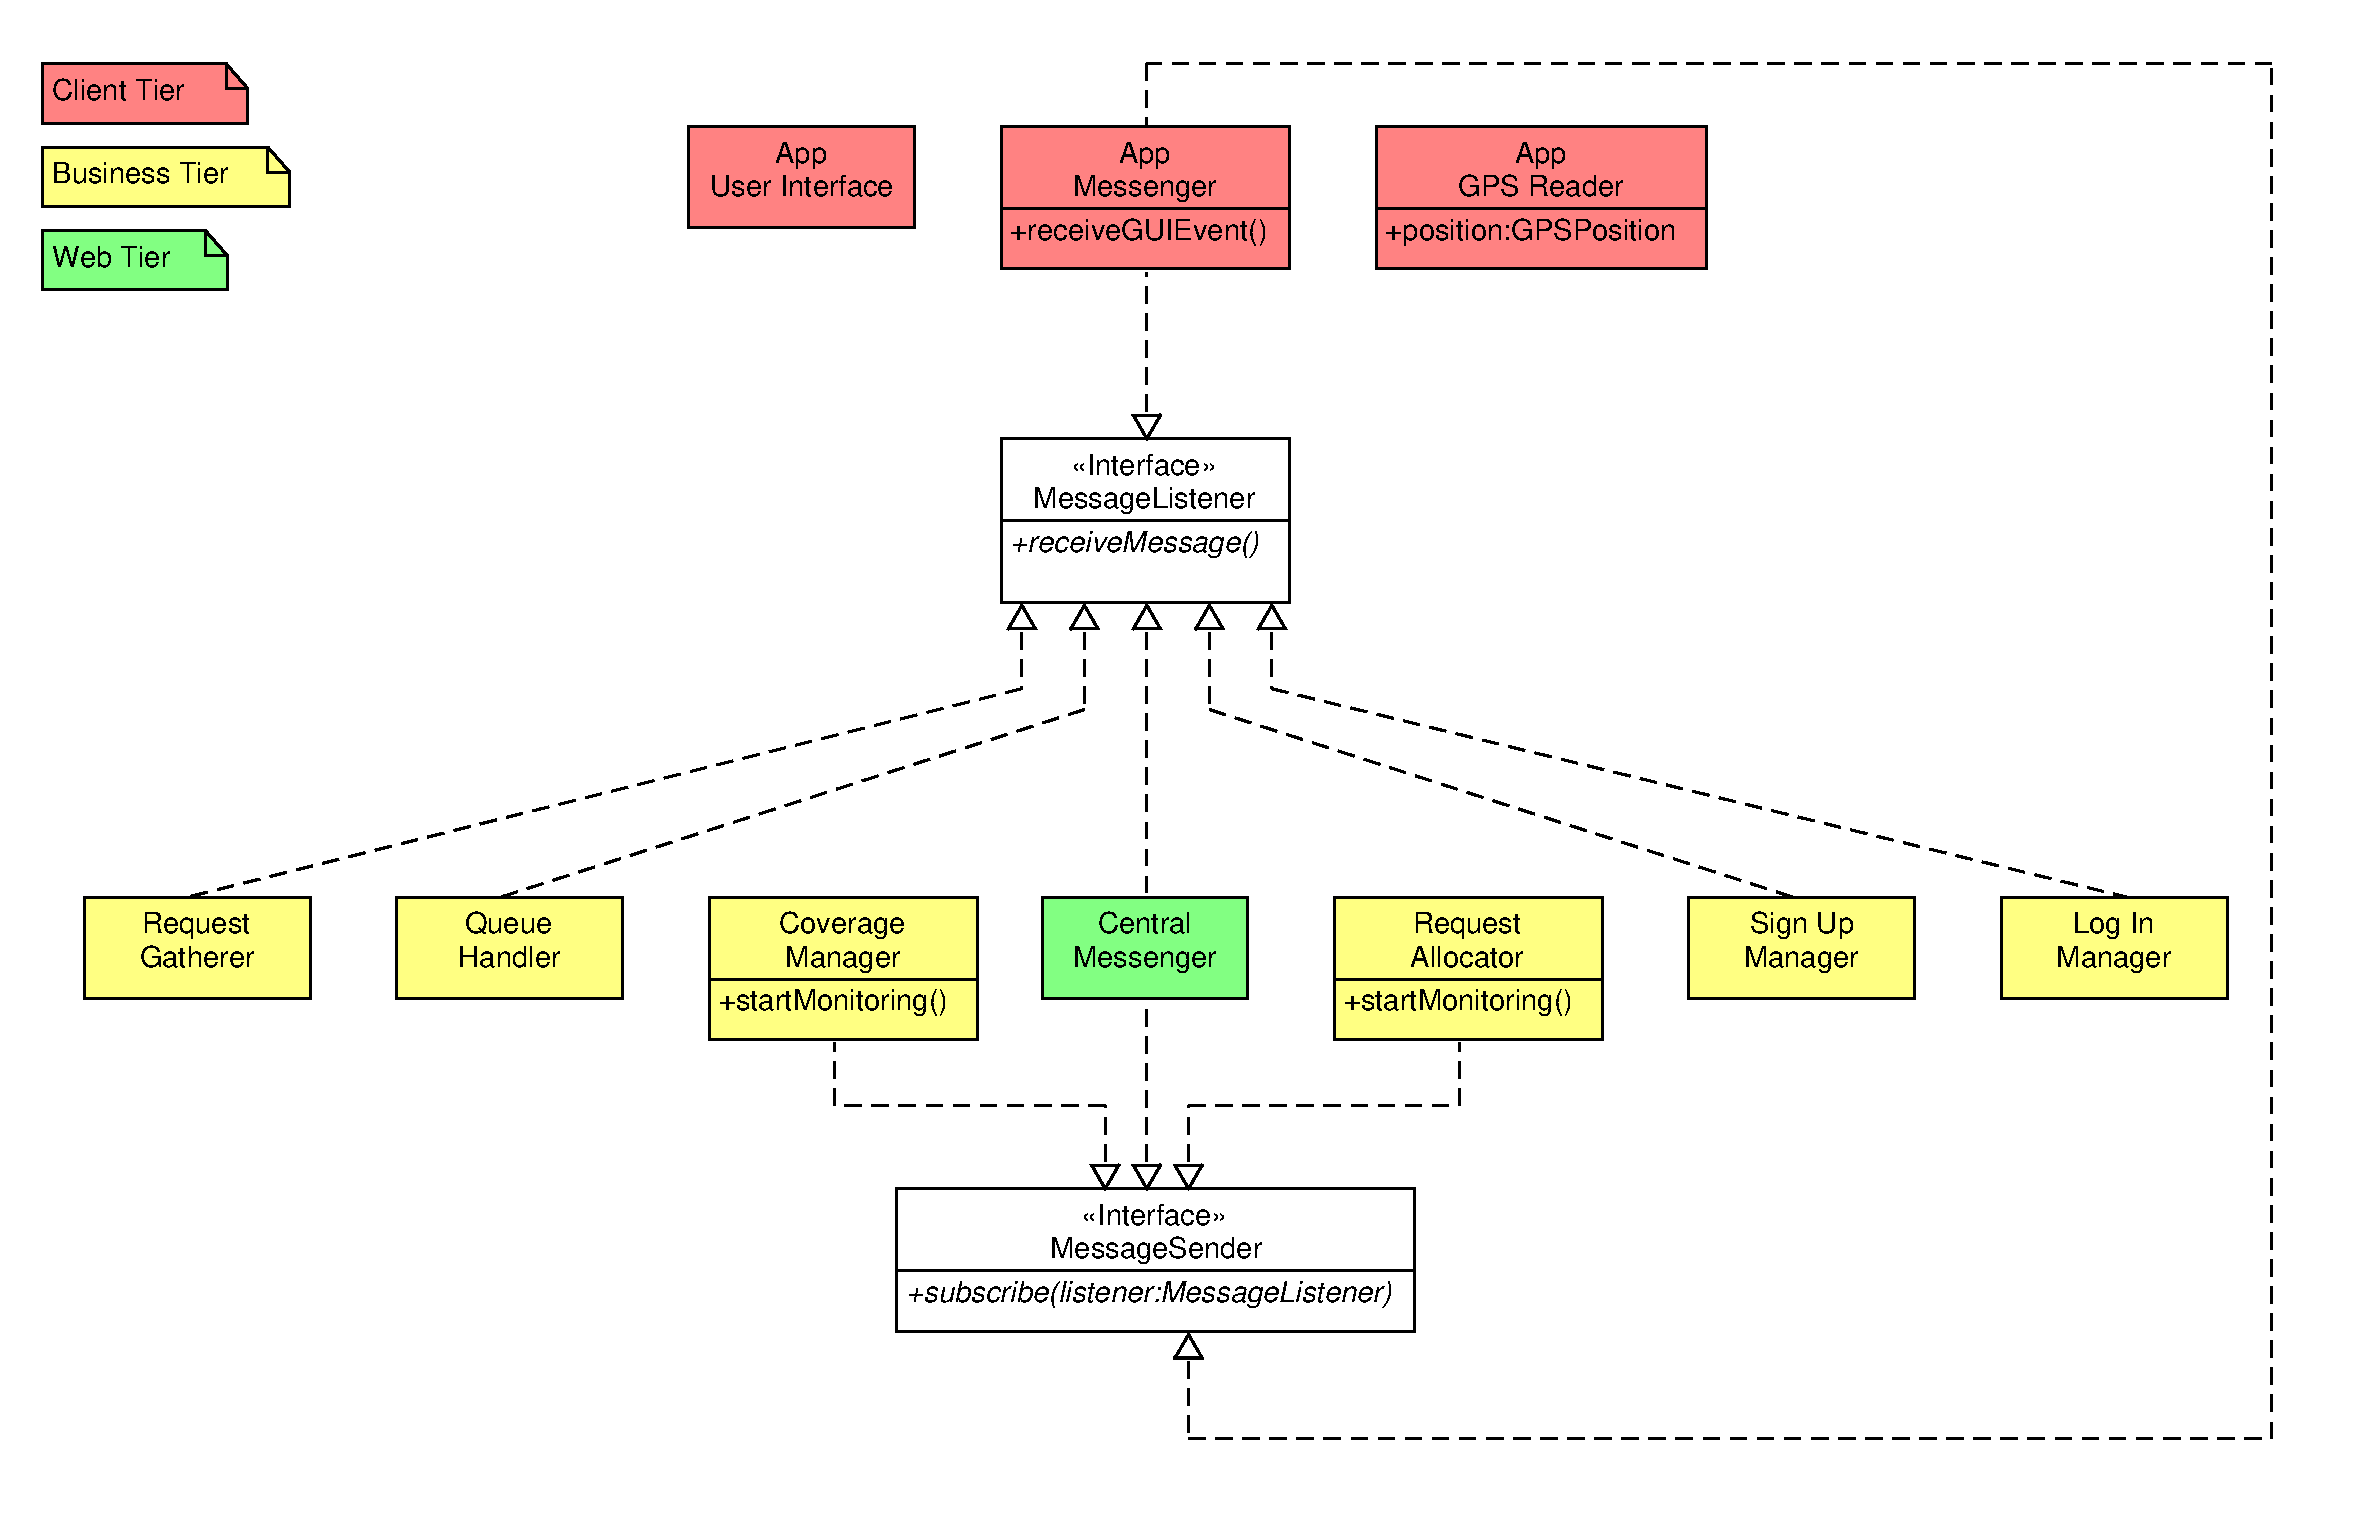
\includegraphics[width=\textwidth]{tex-images/interfaces}
\caption{Component interfaces}
\end{figure}

An Event-based style being used, components have little to no public interfaces to show to the outside world. Every information exchange taking place in the system, any order being given and received, everything is passed along as a \emph{message} event, to which each component, upon inspecting its contents, will react according to what it knows it needs done. As such, every representation of such interfaces is by definition barebone, but a diagram is included for the sake of clarity.

\section{Architectural styles and patterns}


\section{Other design decisions}
